\section{Workflow}
A typical workflow of charge transport simulations is depicted in \fig{workflow}. The first step is the simulation of an \hyperref[sec:morphology]{atomistic morphology}, which is then partitioned on \hyperref[sec:mapping]{hopping sites}. The coordinates of the hopping sites are used to construct a list of pairs of molecules (neighbor list). 

\begin{figure}[h]
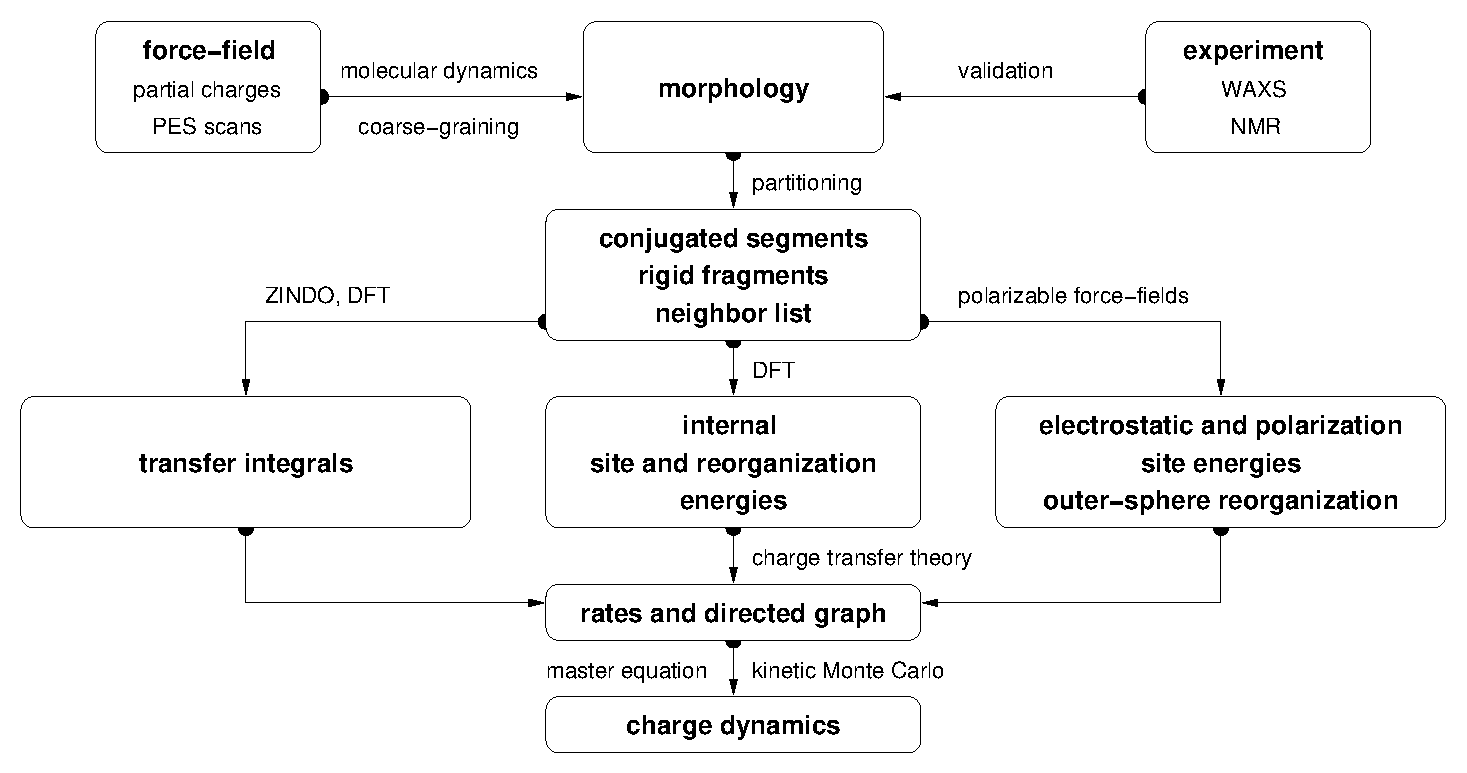
\includegraphics[width=\textwidth]{fig/workflow/workflow}
 \caption{%
   Workflow for microscopic simulations of charge transport.  %
   \label{fig:workflow}}
\end{figure}

For each pair an \hyperref[sec:transfer_integrals]{electronic coupling element}, a reorganization energy, a driving force, and eventually the hopping rate are evaluated. The neighbor list and hopping rates define a directed graph. The corresponding master equation is solved using the  \hyperref[sec:kmc]{kinetic Monte Carlo method}, which allows to explicitly monitor the charge dynamics in the system as well as to calculate time- or ensemble averages of occupation probabilities, charge fluxes, correlation functions, and field-dependent mobilities.
